\section{问题背景}

在这一章节,主要介绍所需加速的神经网络、此类网络在实际问题中的应用和选用的数据集。

\subsection{Relation-Network介绍}

自神经网络迅速发展以来,主要用于解决分类和回归问题,并且已经成功应用到图像、NLP和
语音等多个领域。在此期间,各种类型的网络层出不穷,如:LSTM,CNN和GCN等。

但对于任何神经网络,其准确率和性能都会受到数据数量的影响。当训练数据很少时,网络的
准确率必然会有所下降,而此类问题被称为小样本问题。针对小样本问题,提出了一种新的网络
结构:Relation-Network,采用基于度量的方式来解决小样本问题\cite{RN}。

首先,网络读入支持集中的多组图片,经过特征提取层$f_\phi$得到图片的特征表示$E_1$。
而后读入查询集中的图片,查询集中的图片类别属于支持集多组图片中的某一类。
经过同样的特征提取层(参数一致)$f_\phi$得到另外的特征表示$E_2$。
将查询集的特征表示$E_2$和支持集的特征表示$E_1$拼接到一起,再次经过另外的特征提取层
$g_\phi$得到综合的特征表示$E_3$,最后经过分类层后得到特征向量Relation Score。在Relatoin Score中,
查询集所属的类别的维度得分较高,其他维度得分较低,以此为误差进行反向传播,
模型结构示意图如图\ref{fig:com}所示。

\begin{figure}[ht]
    \centering
    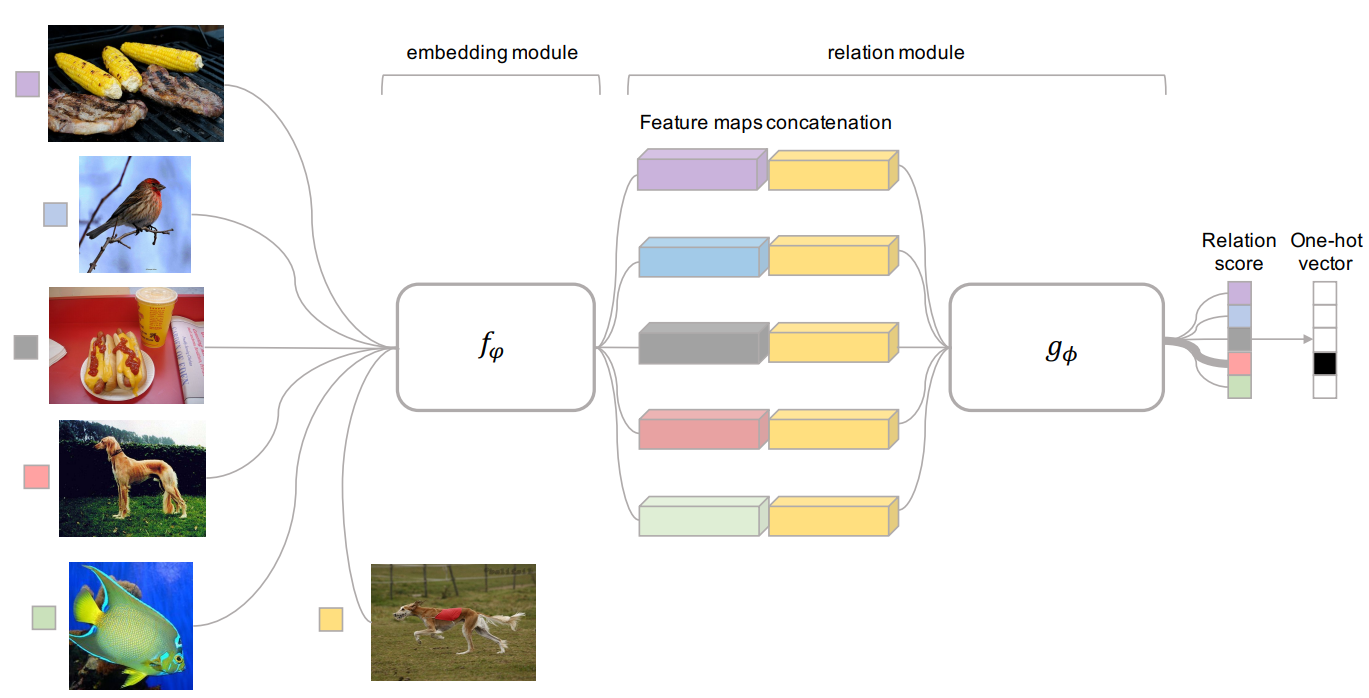
\includegraphics[scale=0.25]{figure/compare.png}
    \caption{Relation-Network网络结构示意图}
    \label{fig:com}
\end{figure}

而选用此网络进行实验的目的是,查询集与支持集的拼接过程难度较大且无法并行化,
来观察在并行受限的情况下是否仍然具有较高的加速比。

\subsection{数据集与选取方法}

miniImageNet\footnote{\ttfamily\scriptsize https://drive.google.com/file/d/0B3Irx3uQNoBMQ1FlNXJsZUdYWEE/view}
数据集含有100个类,每个类有600张三通道彩色图片,
图片的尺寸是$84\times 84$,共。因其类别数量较多,所以miniImageNet
数据集被广泛应用在小样本分类问题中。miniImageNet数据集中的图片实例如图
\ref{mini}所示。

\begin{figure}[h]
    \centering
    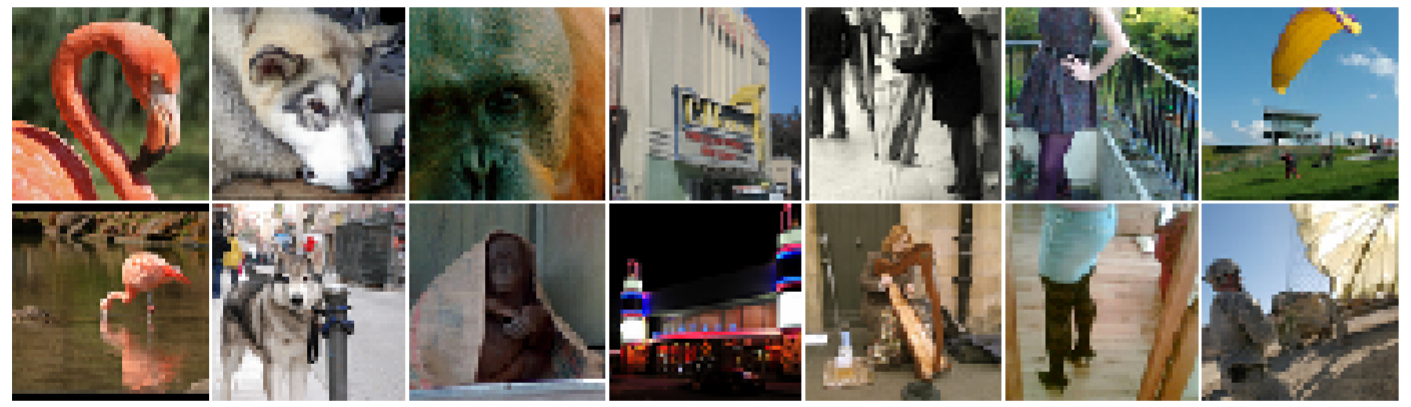
\includegraphics[scale=0.2]{figure/1.png}
    \caption{miniImageNet数据集中的图片实例}
    \label{mini}
\end{figure}

按照小样本问题的标准,网络训练时使用的每组数据由支持集和查询集组成。n\_way表示一组支持集含有类
的数量,k\_query表示查询集中含有的类的数量,k\_shot表示支持集与查询集中每个类有几个样本。

\subsection{模型结构}

因为数据集为彩色图片,所以采用以卷积为主要形式来处理图片,并借助残差块来搭建深层神经网络\cite{dnn}。
最终实现的神经网络中的一个模块包括:卷积层、标准化层和激活函数,以及对输入进行下采样后得到的残差块。模块
结构如图\ref{fig:module}所示:

\begin{figure}[ht]
    \centering
    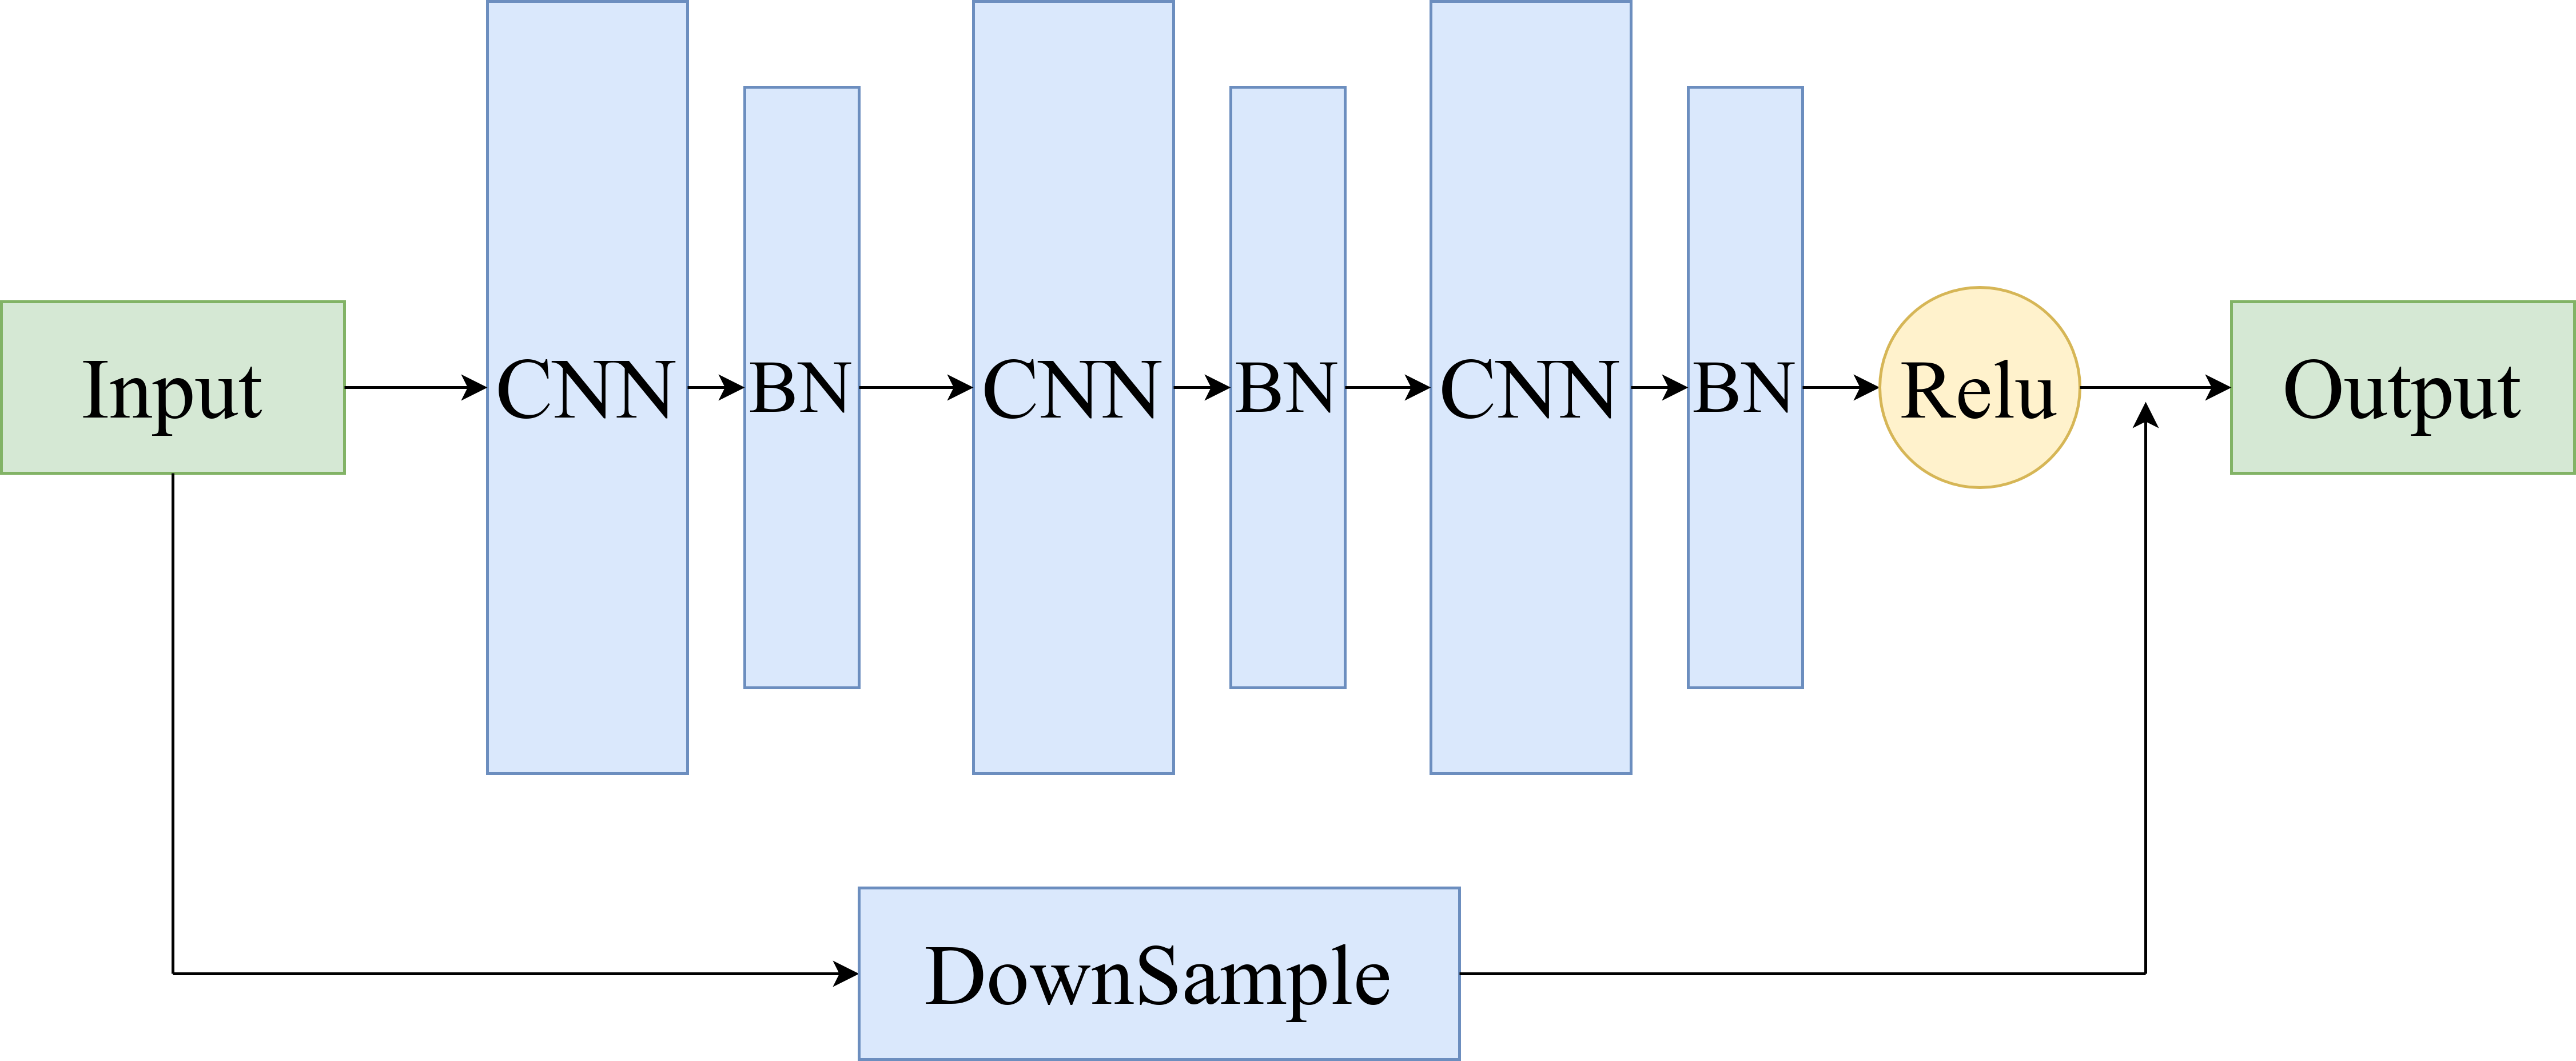
\includegraphics[scale=0.08]{figure/network.png}
    \caption{神经网络中模块结构示意图,CNN表示卷积层,BN表示标准化层,DownSample表示对输入进行下采样,
    Relu表示激活函数,Input表示模块的输入,Output表示模块的输出}
    \label{fig:module}
\end{figure}

$f_\phi$有13组这样的模块,$g_\phi$有7组这样的模块,在网络的最后有一组全连接层,用于计算
查询集的得分:Relation Score。
